\documentclass[11pt]{article}
\usepackage[preprint]{acl}

\usepackage{times}
\usepackage{latexsym}
\usepackage[T1]{fontenc}
\usepackage[utf8]{inputenc}
\usepackage{microtype}
\usepackage{inconsolata}
\usepackage{graphicx}
\usepackage{booktabs}
\usepackage{amsmath}

\title{Assignment 1: Design Doc \\[0.3em]
       {\large Lexical \& Semantic Retrieval on EB-NeRD and MIND}}

\author{Yash More \\
  2024114004 \\
  CS4.406: Information Retrieval \& Extraction}

\begin{document}
\maketitle

\begin{abstract}
This report describes a retrieval pipeline built and measured on two news recommendation
datasets, MIND (English) and EB-NeRD (Danish). Given the articles a user has clicked in the
past, the system retrieves articles they are likely to click next, using two different
approaches: a lexical one based on word overlap (BM25) and a semantic one based on
pre-trained article embeddings. Both are evaluated offline with the official ranking metrics
and submitted to the two Codabench leaderboards. The main finding is that neither approach is
universally better: BM25 wins on MIND and the semantic method wins on EB-NeRD, and the reason
comes down to how good each dataset's provided embeddings are rather than anything inherent to
lexical or semantic retrieval. Alongside accuracy, this report measures the engineering side of
the same choices, comparing the BM25 implementation against an off-the-shelf library, comparing
exact nearest-neighbour search against two approximate indexes, and documenting three real
failures that appeared when the pipeline was run at full test-set scale.
\end{abstract}

\section{Introduction}

\textbf{Background:} A news app has to decide, every time a user opens it, which articles to put in front of them.
The datasets used here record exactly those moments. Each record, called an
\emph{impression}, is one instance of a fixed list of candidate articles being shown to one
user at one timestamp, together with which of those candidates the user actually clicked and
which they ignored. Every impression also carries the list of articles that user had clicked
before that moment, which is the only real signal available about what they are interested in.

\textbf{Two Tasks:} The task, then, is this: given a user's click history as of the moment an impression fired,
find articles they are likely to click, and check the result against what they actually
clicked in that impression. This framing splits naturally into two different jobs, and this
report keeps them separate throughout because they are genuinely different problems. \textbf{The first
is \emph{retrieval}:} searching the entire article catalog, which can be over a hundred
thousand articles, and pulling out a few hundred plausible ones. Here the question is simply
whether the article the user clicked shows up anywhere in that shortlist, which is what
recall@K measures in Sections~\ref{sec:lexical} and~\ref{sec:semantic}. \textbf{The second is
\emph{ranking}:} taking the roughly twenty candidates an impression actually showed and putting
them in the best order. Here the question is whether the clicked one ends up near the top,
which is what AUC, MRR and nDCG measure in Section~\ref{sec:eval}. 
% Real recommender systems are built this way for a practical reason. Scoring every article in the catalog with an expensive model, for every user, on every request is too slow, so a cheap method narrows the catalog down first and a more careful method sorts the survivors.

\textbf{Datasets:} Two datasets are used, and they differ as: MIND is English with about 65,000 articles in the development split; EB-NeRD is
Danish with about 12,000 in the demo split, growing to over 125,000 in the real test set. They
store click history in different shapes, ship different kinds of pre-trained embeddings, and
differ in whether users in the evaluated split have any history at all. Rather than writing
two pipelines, one pipeline is parameterised per dataset, which is what makes the comparisons
in Section~\ref{sec:observations} meaningful: when the two datasets disagree, the difference
comes from the data and not from two separate implementations drifting apart.

\section{Data Pipeline}

Both datasets are parsed into one common format so that everything downstream can be written
once. 
% Articles become a table of identifiers, titles, abstracts or subtitles, categories and tagged entities. Impressions become a table of identifiers, users, timestamps, the candidate list shown, the click labels for those candidates, and the user's click history. 
The two raw formats of the two datasets are quite different: MIND stores a user's history directly inside every impression row as a space-separated string of article identifiers, with no timestamps
attached. EB-NeRD keeps history in a separate file with one row per user, joined onto
impressions by user identifier, and it does record a timestamp for every historical click.
That asymmetry matters later, because it means EB-NeRD could in principle support
time-decayed history weighting while MIND structurally cannot. The 

The train, validation and test splits are drawn by time and never at random. This is the single
most important correctness decision in the pipeline. 
% If the split were random, a click a user made on Thursday could end up in the history feature attached to an impression from Tuesday, which means the model would be given the future while predicting the past. Offline scores would look strong and would not survive contact with a live system, where only the past is ever available. 
For MIND, the training file is cut by calendar day into train and validation,
and the separate development file is held out entirely as the offline test set. For EB-NeRD,
the provided train and validation windows are kept as they are. An automated test asserts, on
every split, that the latest click timestamp in any user's history comes before the earliest
impression timestamp in that split, so this property is checked mechanically rather than
assumed.

The feature store is deliberately small. It holds one article table per dataset, which also
carries the number of times each article was clicked during training, and one user table per
split. The training click counts serve a specific purpose. When a user has no usable history,
neither retrieval method has anything to build a query from, so the system falls back to
ranking by training-set popularity instead of returning an all-zero score row. On MIND this
fallback is used often, since about 14\% of evaluated impressions have empty history.
On EB-NeRD it is never used, because every evaluated user has prior history.

\section{Lexical Retrieval}
\label{sec:lexical}

The lexical method works on the simple idea that if a user has been reading articles about a
topic, other articles containing the same words are probably worth showing them. Concretely,
the titles of the last $N$ articles a user clicked are joined together into one string, and
that string is used as a search query against the titles and abstracts of every article in the
catalog. The scoring function is BM25, which is a refinement of plain word counting that adds
three corrections. (i) Rare words count for more than common ones. (ii) Repeated words help with diminishing
returns, so an article mentioning a word ten times is not treated as ten times more relevant
than one mentioning it once. (iii) Longer articles are penalised slightly, so they do not win just
by containing more words overall. The doc-side part of this score, for every article and
word pair, is
\[
W[d,t] = idf(t)\cdot\frac{tf(t,d)\,(k_1+1)}{tf(t,d) + k_1\!\left(1-b+b\,\frac{L_d}{\bar L}\right)},
\]
where $tf(t,d)$ counts word $t$ inside article $d$, $idf(t)$ measures how rare $t$ is across
the catalog, $L_d$ is the article's length, $\bar L$ the average length, and $k_1=1.5$ and
$b=0.75$ are the usual constants controlling saturation and length penalty.

This was implemented directly rather than taken from a library. Every article-word weight is
computed once into a sparse matrix $W$ with one row per article and one column per vocabulary
word, which for MIND is 65,238 by 60,849 and is only 0.04 percent filled. Scoring a whole
batch of queries is then a single sparse matrix multiplication, and the pattern of non-zero
entries in that matrix is exactly the inverted index the assignment asks for. The obvious
alternative, the \texttt{rank\_bm25} package, was rejected on a measured comparison rather than
a guess. Scoring 196 real queries against MIND's catalog took 73.0 seconds with
\texttt{rank\_bm25}, which scores one article at a time in a Python loop, against 0.09 seconds
with the matrix version: a speedup of about 782 times. Projected to MIND's full test split of
73,152 impressions, the library would need roughly 7.6 hours where this implementation needs
35 seconds. On EB-NeRD, with its smaller catalog, the gap is still about 497 times.

Tokenisation is language-aware, because a tokeniser that strips non-ASCII characters would
destroy Danish words containing \ae{}, \o{} and \aa{}. Both languages use Unicode-aware
splitting with their own stopword lists. Whether to also apply stemming, which reduces words
to their root form so that ``election'' and ``elections'' match, was tested rather than
assumed, and the answer turned out to depend on the language. Stemming helps EB-NeRD
noticeably, raising Pool B recall@200 from 0.0444 to 0.0604, a relative gain of 36 percent,
which fits the fact that Danish builds long compound words that a stemmer can break down. It
slightly hurts MIND, dropping the same measure from 0.1405 to 0.1372. Stemming is therefore
left off by default, since a single global setting would help one dataset and harm the other,
and it was not switched on for the scored submission because doing so would have cost a
resubmission against EB-NeRD's five-per-day limit close to the deadline.

Recall@K is reported under two different candidate pools, shown in Table~\ref{tab:bm25recall},
because a single number would hide what is being asked. Pool A searches the full article
catalog and measures true retrieval power. Pool B restricts the search to articles that
appeared in some impression during the evaluated window, which is closer to what a production
system does when it re-ranks a slate that has already been filtered. Pool B recall is much
higher than Pool A at every cutoff, confirming that the distinction is not merely academic.
The absolute numbers are small in both cases, which is expected: finding one specific article
out of tens of thousands using nothing but the titles a user previously read is a hard problem,
and these are candidate generation numbers, not final ranking quality.

\begin{table*}[t]
\centering
\begin{tabular}{lrrrrrr}
\toprule
 & A@50 & A@100 & A@200 & B@50 & B@100 & B@200 \\
\midrule
MIND (BM25) & 0.80\% & 1.53\% & 2.63\% & 4.88\% & 7.19\% & 10.80\% \\
EB-NeRD (BM25) & 1.01\% & 1.63\% & 2.35\% & 3.32\% & 9.83\% & 30.50\% \\
\bottomrule
\end{tabular}
\caption{BM25 recall@K under both candidate pools. Pool A searches the full article catalog.
Pool B searches only articles that were shown in some impression during the evaluated window.
Pool B is consistently easier, since it is a much smaller and already-filtered set.}
\label{tab:bm25recall}
\end{table*}

\section{Semantic Retrieval}
\label{sec:semantic}

The lexical method can only match articles that literally share words, so it misses an article
about the same topic written with different vocabulary. The semantic method addresses this by
representing each article as a vector of numbers positioned so that articles about similar
things sit close together, and then looking for the articles closest to a vector built from the
user's history. Following an explicit instruction to avoid training or running an embedding
model, only embeddings shipped with the datasets are used. MIND provides
\texttt{entity\_embedding.vec}, which contains 100-dimensional vectors for named entities such
as people and organisations, keyed by Wikidata identifier; an article vector is the average of
the vectors of the entities tagged in its title and abstract, which covers 87.03 percent of the
catalog, with the rest having no tagged entity and therefore no vector at all. EB-NeRD provides
a 300-dimensional word2vec document vector for every article, covering the catalog completely.

Search uses the FAISS library's \texttt{IndexFlatIP}, which computes inner products between
the query vector and every article vector. Because all vectors are normalised to unit length,
this inner product is exactly cosine similarity. This index is exact, meaning it compares
against every article and is guaranteed to return the true nearest neighbours. A plain numpy
implementation is used as a fallback when FAISS is not installed; since the FAISS index is
exact rather than approximate, the fallback returns identical results and is not a degradation.

A user's query vector is the average of the embeddings of their last $N$ clicked articles. The
sweep over $N$ on the validation split chose $N=1$ for the semantic method on both datasets,
against $N=20$ for BM25 on MIND, and the reason is worth stating because it is not obvious.
Averaging many embeddings pulls the result toward the middle of everything the user has ever
read, which describes them in general but not what they want right now. A single most recent
click is a sharper signal. BM25 does not suffer from this, because adding more history words
to a text query only creates more chances to match rather than blurring a single point in
space.

Semantic recall@K is shown in Table~\ref{tab:semrecall}. Comparing it against
Table~\ref{tab:bm25recall} gives a mixed picture. BM25 is better at every cutoff on MIND. On
EB-NeRD the semantic method is better throughout Pool A and at Pool B cutoff 50, but BM25
overtakes it from cutoff 100 onward, and by cutoff 200 BM25 is more than twice as good. This is
a useful reminder that recall@K over the whole catalog and the ranking metrics in
Section~\ref{sec:eval} are different questions, so a method leading on one need not lead on
the other.

\begin{table*}[t]
\centering
\begin{tabular}{lrrrrrr}
\toprule
 & A@50 & A@100 & A@200 & B@50 & B@100 & B@200 \\
\midrule
MIND (semantic) & 0.34\% & 0.51\% & 0.97\% & 2.11\% & 3.68\% & 6.41\% \\
EB-NeRD (semantic) & 1.09\% & 2.14\% & 3.97\% & 4.26\% & 7.68\% & 14.40\% \\
\bottomrule
\end{tabular}
\caption{Semantic recall@K under the same two pools as Table~\ref{tab:bm25recall}. BM25 leads
at every cutoff on MIND. On EB-NeRD the semantic method leads in Pool A and at B@50, but BM25
overtakes it at B@100 and beyond.}
\label{tab:semrecall}
\end{table*}

Exact search is fast enough at these dataset sizes, running at roughly 1140 queries per second
on MIND and 2580 on EB-NeRD at cutoff 200, so there is no practical reason to approximate here.
It is still worth knowing what approximate indexes would buy at larger scale, so both were
measured against exact search rather than left as an assumption. Table~\ref{tab:ann} reports
the result. Both approximate indexes are more than ten times faster than exact search while
still returning over ninety percent of the same top-100 articles. This is not needed at
present scale, but it is exactly the option available when the catalog grows, since exact
search costs time proportional to the number of articles on every single query.

\begin{table}[t]
\centering
\small
\begin{tabular}{llrr}
\toprule
Dataset & Index & Queries/s & Agreement \\
\midrule
MIND    & Exact          &  3{,}624 & 1.000 \\
MIND    & IVF (nprobe 8) & 46{,}476 & 0.913 \\
MIND    & HNSW (ef 64)   & 31{,}940 & 0.931 \\
\midrule
EB-NeRD & Exact          &  2{,}150 & 1.000 \\
EB-NeRD & IVF (nprobe 8) & 43{,}153 & 0.925 \\
EB-NeRD & HNSW (ef 64)   & 40{,}075 & 0.992 \\
\bottomrule
\end{tabular}
\caption{Approximate nearest-neighbour indexes against exact search. Agreement is the fraction
of the exact index's top-100 that the approximate index also returns. Both approximate options
run over ten times faster while still finding more than ninety percent of the same articles.}
\label{tab:ann}
\end{table}

\section{Evaluation Harness}
\label{sec:eval}

The evaluation harness answers the ranking question rather than the retrieval question. For
each impression it takes only the candidates that impression actually showed, scores them with
whichever method is being evaluated, sorts them, and measures how well the clicked candidate
was placed. Four accuracy metrics are used. AUC asks whether a randomly chosen clicked
candidate scores above a randomly chosen unclicked one, so 0.5 means the ranking is no better
than shuffling. MRR looks only at the position of the first clicked candidate and rewards
putting it first. nDCG at cutoffs 5 and 10 rewards placing clicked candidates near the top of
the visible list, with a discount that falls off with position. Every metric is reported with a
bootstrap 95 percent confidence interval computed from 1000 resamples with a fixed seed, so
that small differences between methods can be judged rather than over-read.

Accuracy alone does not describe a recommender fully, so three further metrics are computed
over each impression's top ten. Intra-list diversity measures how different the recommended
articles are from each other, computed both from categories and from embeddings, and guards
against a system that recommends ten near-identical articles. Novelty measures how obscure the
recommendations are, using inverse training popularity, and guards against a system that just
recommends whatever is already popular. Coverage measures what fraction of the catalog ever
appears in anyone's top ten, and guards against a system that keeps recommending the same small
set. Table~\ref{tab:beyond} reports these.

Results are also broken down by slice, since an average can hide a method being good for one
group and bad for another. The two slices are cold-start against warm users, split by whether a
user has fewer than five prior clicks, and head against tail articles, split at the 90th
percentile of training click count. The head and tail split needed care: on both datasets more
than 90 percent of articles have exactly zero training clicks, so the 90th percentile lands on
zero, and a naive comparison of ``at least zero'' would have labelled every article as popular
and left the tail slice empty. A strict greater-than comparison fixes this, and a regression
test now guards it.

\begin{table*}[t]
\centering
\small
\begin{tabular}{lrrrrrrrr}
\toprule
 & AUC & MRR & nDCG@5 & nDCG@10 & ILD (cat.) & ILD (emb.) & Novelty & Coverage \\
\midrule
MIND / BM25        & \textbf{0.554} & \textbf{0.306} & \textbf{0.280} & \textbf{0.342} & \textbf{0.843} & \textbf{0.747} & 16.99 & \textbf{0.055} \\
MIND / semantic    & 0.536 & 0.274 & 0.252 & 0.314 & 0.827 & 0.664 & \textbf{17.03} & 0.049 \\
EB-NeRD / BM25     & 0.501 & 0.267 & 0.283 & 0.383 & \textbf{0.799} & \textbf{0.181} & 14.35 & \textbf{0.148} \\
EB-NeRD / semantic & \textbf{0.509} & \textbf{0.325} & \textbf{0.354} & \textbf{0.439} & 0.781 & 0.171 & \textbf{14.40} & 0.139 \\
\bottomrule
\end{tabular}
\caption{Ranking accuracy and beyond-accuracy metrics on the offline test split, with the
better value per dataset in bold. BM25 wins every accuracy metric on MIND; the semantic method
wins every accuracy metric on EB-NeRD. Diversity and coverage favour BM25 on both datasets,
while novelty is essentially tied.}
\label{tab:beyond}
\end{table*}

Both submissions were generated from these same scoring functions and uploaded to their
respective Codabench leaderboards. Figure~\ref{fig:leaderboards} shows the scored results.

\begin{figure*}[t]
\centering
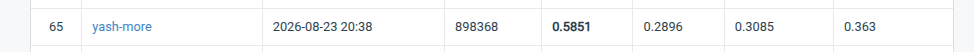
\includegraphics[width=0.92\linewidth]{./screenshots/mind_screenshot.png}\\[4pt]

\includegraphics[width=0.92\linewidth]{./screenshots/eb-nerd_screenshot.png}
\caption{Scored submissions on both Codabench leaderboards. Top: MIND, AUC 0.5851. Bottom:
EB-NeRD, AUC 0.514. Both were produced by the same shared scoring code used for the offline
evaluation.}
\label{fig:leaderboards}
\end{figure*}

\section{Observations}
\label{sec:observations}

The clearest result, visible in Table~\ref{tab:beyond}, is that the two datasets disagree about
which method is better, and they disagree consistently across every accuracy metric. BM25 wins
on MIND and the semantic method wins on EB-NeRD. The temptation is to read this as evidence
about lexical versus semantic retrieval in general, but the more likely explanation is about
the embeddings each dataset happens to provide. EB-NeRD's word2vec vectors were trained on the
same Danish news corpus the articles come from and cover every article, so they genuinely
describe article content. MIND's vectors describe named entities rather than articles, cover
only 87 percent of the catalog, and are being asked to represent an article by averaging
whatever people and organisations it happened to mention. That is a much weaker signal, and it
is competing against BM25 in English, where exact word matching already works well. A fair
summary is that the semantic method wins when it is given good embeddings and loses when it is
not.

The second observation concerns which users each method serves well. On MIND, BM25 improves
from 0.520 AUC on cold-start users to 0.560 on warm users, which is what should happen: more
history means a longer query and more chances to match. The semantic method barely moves,
going from 0.527 to 0.538, and is actually the better of the two on cold-start users
specifically. This fits the earlier finding that averaging many embeddings blurs the signal, so
the semantic method gains little from extra history and can even be hurt by it.

The third observation is the most interesting, and it concerns popular articles. On MIND, BM25
does clearly better on head articles than on tail ones, reaching 0.586 AUC and 0.412 MRR on the
popular tenth of the catalog. The semantic method goes the other way, dropping to 0.476 AUC on
head articles, which is below random, while managing 0.543 on the tail. On EB-NeRD the pattern
splits between metrics rather than between methods: on head articles the semantic method has
better AUC, 0.551 against 0.495, but clearly worse MRR, 0.295 against 0.433. Read together,
this says the semantic method is good at judging which candidates are broadly plausible but
less reliable at picking the single right one, while BM25 is comparatively better at nailing
the exact top position on well-known articles. A production system built on data like this
would probably combine them, using semantic scores for overall ordering with a lexical or
popularity signal to break ties at the very top.

A fourth observation comes from the beyond-accuracy columns in Table~\ref{tab:beyond}, and it
runs against the usual assumption that accuracy and diversity trade off against each other.
BM25 has both higher accuracy on MIND and higher diversity and coverage on both datasets. The
gap in embedding-based diversity on EB-NeRD is striking, 0.181 against 0.171 in absolute terms
but both far below MIND's 0.747 and 0.664, which reflects that EB-NeRD's word2vec vectors place
all articles from one newspaper much closer together than MIND's entity vectors do. Coverage is
low everywhere, 5 percent on MIND and 15 percent on EB-NeRD, meaning most of the catalog never
reaches anyone's top ten. That is expected for content-similarity retrieval with no
exploration mechanism, and it is the kind of thing that would need addressing before deploying
such a system.

\section{Serving-Feature Ablation}
\label{sec:ablation}

A model can look excellent offline by using information that would not exist at the moment a
real prediction has to be made. This section measures how much of an apparently strong result
would come from exactly that. The ablation is run on EB-NeRD only, and not by choice: MIND's
raw files simply do not carry engagement or post-interaction statistics, so the corresponding
columns are entirely empty and the comparison cannot be constructed there at all.

Three configurations are compared, each adding to the previous one, with results in
Table~\ref{tab:ablation}. The clean configuration uses only the retrieval score and is the one
that could actually be deployed. The popularity configuration adds article statistics such as
total views, total read time and sentiment score. These are unavailable at serving time
because they are aggregated over an article's entire lifetime, which includes the future
relative to any particular impression. The post-interaction configuration adds a large bonus
directly to whichever candidate was the true click, which is the most direct leak possible
since the click outcome is the very thing being predicted.

The results are stark. Popularity lifts AUC by roughly 0.07 to 0.08 on both methods, a real and
tempting improvement, since popular articles genuinely do get clicked more. The
post-interaction configuration scores a perfect 1.000 on every metric for both methods, by
construction. The gap between the clean row and the popularity row is the useful number here:
it quantifies how much of a strong-looking popularity-boosted score would be leakage rather
than retrieval quality. Only the clean row is a system; the other two exist to measure the
temptation.

One detail found while building this is worth recording, because it shows that not every leaky
column is actually exploitable. EB-NeRD also ships next read time and next scroll percentage,
which clearly describe what happened after an impression. But these are recorded once per
impression rather than once per candidate, so every candidate in an impression would receive
the same value. Since AUC, MRR and nDCG all depend only on the relative ordering of candidates
within an impression, a value identical across all of them cannot change any of these metrics
at any weight. These columns were therefore not used, and reporting why is more honest than
silently omitting them.

\begin{table}[t]
\centering
\small
\begin{tabular}{llrrr}
\toprule
Method & Configuration & AUC & MRR & nDCG@10 \\
\midrule
BM25     & clean            & 0.501 & 0.267 & 0.383 \\
BM25     & + popularity     & 0.576 & 0.360 & 0.475 \\
BM25     & + post-inter.    & \textbf{1.000} & \textbf{1.000} & \textbf{1.000} \\
\midrule
Semantic & clean            & 0.509 & 0.325 & 0.439 \\
Semantic & + popularity     & 0.581 & 0.363 & 0.479 \\
Semantic & + post-inter.    & \textbf{1.000} & \textbf{1.000} & \textbf{1.000} \\
\bottomrule
\end{tabular}
\caption{Serving-feature ablation on EB-NeRD, 11,798 impressions. Each configuration adds to
the one above it. Only the clean rows are deployable. The perfect scores in the last row of
each block are produced by construction and are worthless, which is precisely the point.}
\label{tab:ablation}
\end{table}

\section{Where It Breaks at Scale}
\label{sec:scale}

This section did not require extrapolation, because the real Codabench test sets are already an
order of magnitude larger than the development data and running against them broke the pipeline
three separate times. EB-NeRD grows from 11,800 articles and 24,700 impressions in the demo
split to 125,500 articles and 13.5 million impressions in the test set, which is 548 times more
impressions. MIND grows from 65,000 articles and 73,000 impressions to 121,000 articles and
2.37 million impressions.

The first failure was memory. Reading the full behaviors and history parquet files into pandas
before any batching, including many columns the pipeline never uses such as device type, scroll
percentage and session identifier, reached 10.5 GB of resident memory on a 15 GB machine and
was killed by the operating system. The fix was to read only the four columns actually needed
and to stream the impressions in batches rather than materialising all 13.5 million rows at
once, which brought peak memory down to 1.7 GB.

The second failure was a data structure chosen for convenience at small scale. The scoring code
built a dictionary mapping every article in the catalog to its score, once per impression. At
MIND's development size this is harmless. At 125,500 articles and 13.5 million impressions,
where each impression only has about twelve real candidates, it was estimated at more than 70
hours of pure dictionary construction, entirely separate from the actual arithmetic. The fix
was to build the dictionary only over each batch's own candidates, using a precomputed mapping
from article identifier to matrix column.

The third failure was the arithmetic itself. Even after the previous fix, computing the full
similarity matrix between each batch and the entire catalog took an estimated 10 hours,
measured at 367 impressions per second. The key realisation is that the columns of that matrix
are independent of one another, so restricting the multiplication to only the 250 to 300
distinct candidate columns a batch actually touches produces numerically identical results
rather than an approximation. This was verified: the largest difference between the restricted
and full computations was $1.8\times10^{-7}$, which is ordinary 32-bit floating point rounding.
The run dropped from an estimated 10 hours to 49 minutes, or 4,629 impressions per second.

An earlier version of this report also blamed the slow run partly on the numpy build limiting
OpenBLAS to two threads, based on a \texttt{MAX\_THREADS=2} field printed by numpy's build
configuration. That claim is withdrawn. Sweeping the thread count directly on the real matrix
shape shows performance continuing to improve past two threads, from 180 to 95 to 52
milliseconds at one, two and four threads, plateauing at four, and this was confirmed with a
bare numpy benchmark outside the pipeline. The printed field is not an enforced runtime
ceiling. The genuine bottleneck was matrix size alone. Interestingly, BM25's sparse
multiplication shows no thread sensitivity whatsoever, staying flat at about 2,150 queries per
second from one to eight threads, because scipy's sparse routines do not go through the same
threaded dense-matrix path that numpy's dense multiplication uses. The two needed separate
measurement rather than a shared assumption.

Applying all three fixes preemptively when writing MIND's submission script produced a clean
first run at 0.83 GB of memory and 2,019 impressions per second. A fourth problem was unrelated
to any of this: downloading EB-NeRD's 1.6 GB test set over a single connection crawled at 15 to
30 KB/s with repeated stalls, reproduced from two different networks, while the same machine
reached 1.5 MB/s to a different host. A single connection's throughput is limited by packet
loss and round-trip time rather than by the link's capacity, so splitting the download across
24 parallel range requests raised effective throughput roughly thirtyfold.

Looking further ahead, EB-NeRD's full production data is around 600 million impressions, about
44 times beyond what was tested here. Even the fixed scoring loop would need roughly 36 hours
at that size, because once the matrix multiplication is no longer dominant the per-impression
Python loop that sorts ranks and looks up dictionary entries becomes the bottleneck. That would
need either sharding across processes and machines or replacing the per-row loop with a fully
vectorised ranking operation. BM25's dense-matrix materialisation step, which worked at MIND's
2.37 million scale, would need the same candidates-only restriction at EB-NeRD's full size.
Article embeddings held in memory stay manageable at ten times the catalog size, around 1.5 GB,
but would need streaming at a hundred times. And the parallel downloader is a workaround rather
than a fix: at ten times the data volume, a genuinely bad network path needs a regional mirror
or pre-staged shared storage, not more connections from one machine.

\section{Limitations}

Everything here runs on a single machine with no GPU. Embeddings are used as provided rather
than trained, which was an explicit instruction and which trades representation quality for
zero training cost and full reproducibility, but it does mean the semantic method's ceiling is
set by whatever each dataset happened to ship. The approximate nearest-neighbour comparison in
Table~\ref{tab:ann} was measured at development scale only, not at the larger catalog sizes
where it would actually matter. Cold-start handling is limited to falling back on training
popularity, with no exploration or content-based bootstrapping. Stemming was measured and found
to help EB-NeRD but was not adopted into the scored submission, so the leaderboard number is
from the unstemmed configuration. Finally, both Codabench test sets are genuinely blind, so
submissions could only be checked structurally offline and their real quality was unknown until
the leaderboards scored them.

\section*{References}

\begingroup
\small
\setlength{\parindent}{-1em}
\leftskip=1em
\setlength{\parskip}{2pt}

Wu, F., Qiao, Y., Chen, J.-H., et al. 2020. MIND: A Large-scale Dataset for News
Recommendation. \emph{ACL 2020}.

Kruse, J., Lindskow, K., Kalloori, S., et al. 2024. EB-NeRD: A Large-Scale Dataset for News
Recommendation. \emph{RecSys Challenge 2024}.

Robertson, S. and Zaragoza, H. 2009. The Probabilistic Relevance Framework: BM25 and Beyond.
\emph{Foundations and Trends in Information Retrieval}.

Johnson, J., Douze, M. and J\'egou, H. 2019. Billion-scale Similarity Search with GPUs.
\emph{IEEE Transactions on Big Data}.
\par
\endgroup

\end{document}
